%31/03 - Carlos Alaíz 
\chapter{Modelos lineales, métodos de Kernel y redes neuronales}
\section{Modelos lineales de regresión}
El aprendizaje supervisado es la creación de un modelo que prediga la salida en base a unas entradas, partiendo de un histórico con parejas entrada-salida. Dentro de esto aparece la regresión, donde se quiere predecir un valor continuo. 

Los elementos de un problema de aprendizaje supervisado son:
\begin{itemize}
\item Datos: parejas entrada-salida
\item Características: atributos
\item Objetivo: la salida real, las etiquetas, la salida asociada
\item Modelo: una función matemática de x a y que proporciona la salida. Puede tener varios parámetros $\Theta$.
\item Algoritmo de aprendizaje: procedimiento para la obtención del modelo en base a los datos.
\end{itemize}

El enfoque más sencillo de la regresión es un modelo constante, ignorando la entrada. Así, se define la salida como una combinación lineal de entradas, creando un modelo lineal. La ventaja es que es simple, robusto, interpretable, fácil de entrenar y fácil de predecir. La desventaja es que sea demasiado limitado y un subajuste a los datos.

\subsection{Regresión lineal 1-dimensional}
El caso más simple tiene un solo dato de valores reales. El modelo lineal simple sería una línea recta con parámetros $\Theta = \{b, w\}$, siendo $b$ el sesgo y $w$ la pendiente de la recta. Así, el modelo se definiría como
$$f_{\Theta} = b + wx$$

Ejercicio: dado este modelo lineal con $b=1$ y $w=2$, computa la salida del modelo para $x=2$ y para $x=-1$.
$$1 + 2 \cdot 2 = 1 + 4 = 5$$
$$1 + 2 \cdot -1 = 1 - 2 = -1 $$

Se necesita un procedimiento que determine el sesgo y la pendiente para optimizar la calidad del modelo. Se pueden utilizar dos perspectivas para definir la calidad: 
\begin{itemize}
\item En base al error: medida sobre cómo de bien se ajusta el modelo a los datos de entrenamiento
\item En base a la complejidad: un término de regulación que penaliza la complejidad del modelo
\end{itemize}

Se define el residuo como la diferencia entre lo que se debería haber predicho y lo que el modelo ha predicho. El error cuadrático sería la esperanza de los residuos al cuadrado. Es decir, sobre el conjunto de datos de entrenamiento, se mide el error, se suma y se eleva al cuadrado. Esto es una medida automática de cuánto se confunde el modelo. También se puede calcular el error absoluto con el valor absoluto en lugar del error cuadrado. 

Ejercicio: calcular MAE y MSE del modelo anterior con $b=1$ y $w=2$ con los pares (2,4) y (-1,1).
$$f_{\Theta} = 1 + 2 \cdot 2 = 1 + 4 = 5 \neq 4$$
$$f_{\Theta} = 1 + 2 \cdot -1 = 1 - 2 = -1 \neq 1$$
$$r = -1, 2$$
$$MAE = 1/2 \cdot (1 + 2) = 1/2 \cdot 3 = 1.5$$
$$MSE = 1/2 \cdot (1^2 + 2^2) = 1/2 \cdot (1 + 4) = 2.5$$

%01/04 - Carlos
\subsubsection{Optimización}
Optimizar hace referencia a encontrar la mejor solución posible respecto a algún criterio. 

En un modelo lineal, hay que elegir una métrica que generalmente es el error cuadrático. Esto se debe a que es diferenciable (se puede calcular la derivada) y tiene sentido geométricamente. En el algoritmo, la optimización sería los valores de $b$ y $w$ que hacen que el error cuadrático sea mínimo.

En resumen, la línea de regresión por mínimos cuadrados se obtiene resolviendo
$$\min_{b, w \in \mathbb{R}} \left\{ \frac{1}{N} \sum_{i=1}^{N} \left( y_i - (b + w x_i) \right)^2 \right\}$$
Los elementos auxiliares son:
$$
\bar{y} = \frac{1}{N} \sum_{i=1}^{N} y_i \quad \text{(Mean Target)}, \quad
\bar{x} = \frac{1}{N} \sum_{i=1}^{N} x_i \quad \text{(Mean Feature)},
$$
$$
\hat{y}_i = y_i - \bar{y} \quad \text{(Centred Target)}, \quad
\hat{x}_i = x_i - \bar{x} \quad \text{(Centred Feature)}.
$$

Ejercicio: dado los siguientes pares de datos (0,4), (1,6), (2,4), (3,6), (4,8), computa:
\begin{itemize}
\item El valor de $\bar{x}$ y $\bar{y}$: 
$$\bar{x} = (0 + 1 + 2 + 3 + 4)/5 = 10/5 = 2$$
$$\bar{y} = (4 + 6 + 4 + 6 + 8)/5 = 28/5 = 5.6$$

\item El valor de $\hat{x}_i$ y $\hat{y}_i$:
$$\hat{x}_1 = 0 - 2 = -2 \quad \hat{y}_1 = 4 - 5.6 = -1.6$$
$$\hat{x}_2 = 1 - 2 = -1 \quad \hat{y}_2 = 6 - 5.6 = 0.4$$
$$\hat{x}_3 = 2 - 2 = 0 \quad \hat{y}_3 = 4 - 5.6 = -1.6$$
$$\hat{x}_4 = 3 - 2 = 1 \quad \hat{y}_4 = 6 - 5.6 = 0.4$$
$$\hat{x}_5 = 4 - 2 = 2 \quad \hat{y}_5 = 8 - 5.6 = 2.4$$

\item El valor de $w^*$ y $b^*$:
$$w^* = \frac{\sum^N_{i=1} \hat{x}_i\hat{y}_i}{\sum^N_{i=1} \hat{x}_i\hat{x}_i} = \frac{3.2 - 0.4 + 0 + 0.4 + 4.8 }{4 + 1 + 0 + 1 + 4} = \frac{8}{10} = 0.8$$
$$b^* = \bar{y} - w^*\bar{x} = 5.6 - 0.8 \cdot 2 = 4$$

\item El valor de MSE:
$$MSE = \frac{1}{N} \sum^N_{i=1} (y_i - (b + wx_i))^2$$
$$\frac{1}{5} \cdot ((4 - (4 + 0.8\cdot 0)^2 + 6 - (4 + 0.8\cdot 1)^2 + 4 - (4 + 0.8\cdot 2)^2 + 6 - (4 + 0.8\cdot 3)^2 + 8 - (4 + 0.8\cdot 4))^2$$
$$\frac{1}{5} \cdot (0 + 1.44 + 2.56 + 0.16 + 0.64) = \frac{1}{5} \cdot 4.8 = 0.96$$
\end{itemize}

\subsection{Regresión lineal múltiple}
Por simplicidad, $\mathcal{X} = \mathbb{R}^d$. Los datos se representan como $D = \{ (x_i, y_i) \}_{i=1}^N$, donde $x_i = (x_{i,1}, x_{i,2}, \ldots, x_{i,d}) \in \mathbb{R}^d$ y $y_i \in \mathbb{R}$.

El modelo lineal correspondiente es un hiperplano, con parámetros $\theta = \{ b, w \}$.
\begin{itemize}
\item $b \in \mathbb{R}$ es el término de intercepción o sesgo.
\item $w = (w_1, w_2, \ldots, w_d) \in \mathbb{R}^d$ es el vector normal del hiperplano.
\item El modelo se define como:    
    $$f_\theta (\mathbf{x}) = b + w^\top \mathbf{x} = b + \sum_{i=1}^d w_i x_i.$$
\end{itemize}

El algoritmo de aprendizaje determinará $b$ y $w$ utilizando $D$.

Ejercicio: dado un modelo lineal bidimensional con parámetros $\Theta = \{ b, \vec{w}\}$ con $b = 1$ y $\vec{w} = (1,2)^T$. Computa la salida del modelo para $\vec{x} = (1,1)^T$:
$$1 + (1 \cdot 1 + 1 \cdot 2) = 4$$
 Computa la salida del modelo para $\vec{x} = (-1,0)^T$:
 $$1 + (1 \cdot -1 + 0 \cdot 2) = 0$$

\subsubsection{Ecuaciones lineales}
Se necesita un procedimiento para determinar el sesgo $b $ y el vector $\mathbf{w}$.

Un primer enfoque es intentar igualar todos los pares entrada-salida $(x_i, y_i)$, $i = 1, \ldots, N$. Específicamente:
$$
\begin{cases}
b + \mathbf{w}^T x_1 = y_1 \\
b + \mathbf{w}^T x_2 = y_2 \\
\vdots \\
b + \mathbf{w}^T x_N = y_N
\end{cases}
\equiv 
\begin{cases}
b + w_1 x_{1,1} + w_2 x_{1,2} + \cdots + w_d x_{1,d} = y_1 \\
b + w_1 x_{2,1} + w_2 x_{2,2} + \cdots + w_d x_{2,d} = y_2 \\
\vdots \\
b + w_1 x_{N,1} + w_2 x_{N,2} + \cdots + w_d x_{N,d} = y_N
\end{cases}
$$

La siguiente notación matricial puede simplificar las ecuaciones:
$$
\mathbf{X} =
\begin{pmatrix}
x_{1,1} & x_{1,2} & \cdots & x_{1,d} \\
x_{2,1} & x_{2,2} & \cdots & x_{2,d} \\
\vdots & \vdots & \ddots & \vdots \\
x_{N,1} & x_{N,2} & \cdots & x_{N,d}
\end{pmatrix}
;\quad \tilde{\mathbf{X}} =
\begin{pmatrix}
1 & x_{1,1} & \cdots & x_{1,d} \\
1 & x_{2,1} & \cdots & x_{2,d} \\
\vdots & \vdots & \ddots & \vdots \\
1 & x_{N,1} & \cdots & x_{N,d}
\end{pmatrix}
;\quad \mathbf{y} =
\begin{pmatrix}
y_1 \\
y_2 \\
\vdots \\
y_N
\end{pmatrix}
;\quad \tilde{\mathbf{w}} =
\begin{pmatrix}
b \\
w_1 \\
\vdots \\
w_d
\end{pmatrix},
$$

donde $\mathbf{X} \in \mathbb{R}^{N \times d}$ es la matriz de datos, $ \tilde{\mathbf{X}} \in \mathbb{R}^{N \times (d+1)}$ es la matriz de datos con un término constante, $\mathbf{y} \in \mathbb{R}^N$ es el vector de objetivos y $\tilde{\mathbf{w}} \in \mathbb{R}^{d+1}$ es el vector de pesos que incluye el intercepto.

El sistema de ecuaciones se convierte en $\tilde{\vec{X}}\tilde{\vec{w}} = \vec{y}$. Como $\tilde{\vec{X}} \in \real^{N \times (d + 1)}, \tilde{\vec{w}} \in \real^{d + 1}$ y $\vec{y} \in \real^N$, tenemos $N$ ecuaciones y $d + 1$ incógnitas. Normalmente, $N >> d+1$ y el sistema está \textbf{sobredeterminado}.

\subsubsection{Calidad del modelo}
Se define con el término de error y de complejidad, al igual que en el caso de una sola dimensión. Los residuos son la desviación de la salida con respecto a la predicción. El error cuadrático y el error absoluto se definen igual que antes.

Para el $i$-ésimo patrón, el \textbf{residual} se define como:
$$
r_i = y_i - f_\theta(\mathbf{x}_i) = y_i - (b + \mathbf{w}^\intercal\mathbf{x}_i).
$$

El \textbf{Error Cuadrático Medio} se calcula como:
$$
\text{MSE}(b, \mathbf{w}) = \mathbb{E}\left[R^2\right] \approx \frac{1}{N} \sum_{i=1}^{N} \big(y_i - (b + \mathbf{w}^\intercal\mathbf{x}_i)\big)^2.
$$

$$
\text{MAE}(b, \mathbf{w}) = \mathbb{E}\left[|R|\right] \approx \frac{1}{N} \sum_{i=1}^{N} \left|y_i - (b + \mathbf{w}^\intercal\mathbf{x}_i)\right|.
$$

Ejercicio: dado un modelo lineal bidimensional con parámetros $\Theta = \{b, \vec{w}\}$, con $b=1$ y $\vec{w} = (1,2)^T$, y los datos siguientes datos para $x_{i,1}$, $x_{i,2}$ y $y_i$, computa MAE y MSE.
Para un modelo lineal bidimensional:
$$f(x_1, x_2) = b + w_1x_1 + w_2x_2$$
En el enunciado nos dicen b y w, por lo que la fórmula queda en:
$$f(x_1, x_2) = 1 + 1 x_1 + 2 x_2$$
Ahora tenemos dos datos, por lo que calculamos las salidas predichas:
$$f_1 = 1 + 1 + 2 = 4$$
$$f_2 = 1 - 1 + 0 = 0 \neq 2$$
Los residuos son 0 y 2. Por tanto, los residuos cuadrados son 0 y 4. Calculando la media, $MAE = 1$ y $MSE = 2$. 

\subsubsection{Optimización basada en gradiente: problemas multidimensionales}
En muchas dimensiones, la derivada se generaliza con el gradiente, que es un vector de derivadas parciales. El gradiente define el hiperplano tangente. 

\subsubsection{Entrenamiento de un modelo lineal}
Usualmente se utiliza como función de error el MSE al ser diferenciable y corresponderse a la distancia entre los vectores de predicción y de salida esperada. Se busca minimizar este error, calculando para cada entrada la salida correspondiente y viendo el error.

El problema de optimización para encontrar los parámetros óptimos se formula como:

$$
\min_{\substack{b \in \mathbb{R} \\ \mathbf{w} \in \mathbb{R}^d}} \left\{ \text{MSE}(b, \mathbf{w}) \right\} = \min_{\substack{b \in \mathbb{R} \\ \mathbf{w} \in \mathbb{R}^d}} \left\{ \frac{1}{N} \sum_{i=1}^{N} \big(y_i - (b + \mathbf{w}^\intercal\mathbf{x}_i)\big)^2 \right\} \equiv \min_{\tilde{\mathbf{w}} \in \mathbb{R}^{d+1}} \left\{ (\mathbf{y} - \tilde{\mathbf{X}}\tilde{\mathbf{w}})^\top (\mathbf{y} - \tilde{\mathbf{X}}\tilde{\mathbf{w}}) \right\}.
$$

Para encontrar el punto óptimo $\tilde{\mathbf{w}}^*$, calculamos el gradiente e igualamos a cero:

$$\nabla_{\tilde{\mathbf{w}}} \text{MSE}(\tilde{\mathbf{w}})\big|_{\tilde{\mathbf{w}}=\tilde{\mathbf{w}}^*} = \mathbf{0} \implies 2\tilde{\mathbf{X}}^\top(\mathbf{y} - \tilde{\mathbf{X}}\tilde{\mathbf{w}}^*) = \mathbf{0}
$$

Esto conduce al sistema de ecuaciones normales:

$$\tilde{\mathbf{X}}^\top \mathbf{y} - \tilde{\mathbf{X}}^\top \tilde{\mathbf{X}}\tilde{\mathbf{w}}^* = \mathbf{0} \\
\implies \tilde{\mathbf{X}}^\top \tilde{\mathbf{X}}\tilde{\mathbf{w}}^* = \tilde{\mathbf{X}}^\top \mathbf{y}
$$

Finalmente, la solución óptima (si $\tilde{\mathbf{X}}^\top \tilde{\mathbf{X}}$ es invertible) es:

$$
\tilde{\mathbf{w}}^* = (\tilde{\mathbf{X}}^\top \tilde{\mathbf{X}})^{-1} \tilde{\mathbf{X}}^\top \mathbf{y} \quad \text{(Mínimos Cuadrados)}
$$

Caso especial: cuando $\tilde{\mathbf{X}}^\top \tilde{\mathbf{X}}$ es invertible y $N = d+1$, se simplifica a:
$$
\tilde{\mathbf{w}}^* = \tilde{\mathbf{X}}^\top \mathbf{y}
$$

En resumen, el modelo de mínimos cuadrados lineales es la solución del siguiente problema de optimización:
$$
\min_{\begin{subarray}{c} 
    b \in \mathbb{R} \\
    \mathbf{w} \in \mathbb{R}^d 
\end{subarray}} \left\{ 
    \frac{1}{N} \sum_{i=1}^{N} \big(y_i - (b + \mathbf{w}^{\intercal} \mathbf{x}_i)\big)^2 
\right\}.
$$

La solución óptima viene dada por:
$$
\begin{pmatrix} b^* \\ \mathbf{w}^* \end{pmatrix} = 
\tilde{\mathbf{w}}^* = 
\tilde{\mathbf{X}}^{\dagger} \mathbf{y} = 
\begin{bmatrix} \mathbf{1} & \mathbf{X} \end{bmatrix}^{\dagger} \mathbf{y},
$$

donde:
\begin{itemize}
\item $\tilde{\mathbf{X}} = \begin{bmatrix} \mathbf{1} & \mathbf{X} \end{bmatrix}$ es la matriz de diseño aumentada
\item $\dagger$ denota la pseudoinversa de Moore-Penrose
\item $\mathbf{1}$ es un vector columna de unos
\end{itemize}

\subsection{Resumen: modelos lineales para regresión}
Un problema de regresión es un problema supervisado con objetivos continuos. Un modelo de regresión sencillo pero útil es el modelo lineal. La predicción es una combinación lineal de las características. Para entrenar el modelo lineal, se suele resolver un problema de optimización. El MSE suele utilizarse para medir la calidad del modelo. Es una elección natural. El problema resultante puede resolverse de forma cerrada utilizando el pseudoinverso de la matriz de datos.

%07/04 - Carlos
\section{Modelos lineales de clasificación}
Un problema de clasificación es un problema de aprendizaje supervisado en el que las salidas son discretas. Ejemplos son predecir si un paciente padece o no una determinada enfermedad en función de datos médicos, distinguir la especie de un pez capturado utilizando los datos proporcionados por varios sensores o discernir el tipo de objeto que aparece en una imagen.

Los elementos de un problema de aprendizaje supervisado son:
\begin{itemize}
\item Datos: conjunto de pares entrada-salida
\item Características: vector de atributos (variables independientes/de entrada, covariables...)
\item Etiquetas: objetivo (variable dependiente, resultado...)
\item Modelo: asignación del espacio de entrada al de salida
\item Algoritmo de aprendizaje: procedimiento para obtener un modelo basado en los datos
\end{itemize}

\subsection{Clasificación binaria lineal}
El escenario de clasificación más importante es cuando M = 2 (clasificación binaria).
Si M > 2, existen técnicas de codificación para transformar el problema en varios subproblemas binarios.
Las clases suelen denominarse C0 y C1, y se representan con una codificación 0/1 (o -1/1). Las etiquetas se transforman en:
$$t_i = \begin{cases}
0 \quad \text{if } y_i = \mathcal{C}_0 \\
1 \quad  \text{if } y_i = \mathcal{C}_1
\end{cases}
$$

Los enfoques más simples de clasificación son:
\begin{itemize}
\item Ignorar la entrada: modelo constante (normalmente, clase mayoritaria).
\item Definir la salida como una combinación lineal de las entradas más una transformación: modelo lineal. Es simple, robusto (varianza pequeña), interpretable, fácil de entrenar y fácil de predecir. No obstante, tiene flexibilidad limitada y un ajuste insuficiente (gran sesgo).
\end{itemize}

Por simplicidad, $\mathcal{X}=\mathbb{R}^{d}$.
Los datos se convierten en $\mathcal{D}=\{(x_{i},t_{i})\}_{i=1}^{N}$, donde $x_{i}=(x_{i,1},x_{i,2},\ldots,x_{i,d})\in\mathbb{R}^{d}$ y $t_{i}\in\{0,1\}$.
El modelo lineal correspondiente es un hiperplano, con parámetros $\boldsymbol{\theta}=\{b,\mathbf{w}\}$.

\begin{itemize}
    \item $b\in\mathbb{R}$ es el término de intercepción o sesgo.
    
    \item $\mathbf{w}=(w_{1},w_{2},\ldots,w_{d})\in\mathbb{R}^{d}$ es el vector normal del hiperplano.
    
    \item El modelo se define como:
    \[f_{\boldsymbol{\theta}}(\mathbf{x})=\begin{cases}
    0 & \text{si } b+\mathbf{w}^{\intercal}\mathbf{x}<0, \\
    1 & \text{si } b+\mathbf{w}^{\intercal}\mathbf{x}\geq 0.
    \end{cases}\]
    
    \item El hiperplano divide el espacio en dos mitades, una para la clase $\mathcal{C}_{0}$ y la otra para la clase $\mathcal{C}_{1}$.
\end{itemize}

El \textbf{algoritmo de aprendizaje} determinará $b$ y $\mathbf{w}$ utilizando $\mathcal{D}$.

Ejercicio: dado un modelo de clasificación lineal binario bidimensional con parámetros $\theta = \{b, \vec{w}\}$, con $b = 1$ y $\vec{w} = (1, 2)^T$:
\begin{itemize}
\item Calcula la salida del modelo para $\vec{x}_1 = (1,1)$:

$$1 + 1 \cdot 1 + 2 \cdot 1 = 4 \rightarrow f_{\theta}(\vec{x}) = \mathcal{C}_1$$

\item Calcula la salida del modelo para $\vec{x}_2 = (1,-2)$:

$$1 + 1 \cdot 1 + 2 \cdot (-2) = -2 \rightarrow f_{\theta}(\vec{x}) = \mathcal{C}_0$$

\item Calcula la salida del modelo para $\vec{x}_3 = (0,0)$:

$$1 + 1 \cdot 0 + 2 \cdot 0 = 1 \rightarrow f_{\theta}(\vec{x}) = \mathcal{C}_1$$
\end{itemize}

\subsubsection{Calidad del modelo}
Se necesita un procedimiento para determinar el sesgo $b$ y el vector $w$, optimizando la calidad del modelo. Hay que definir la calidad del modelo. Normalmente desde dos puntos de vista:
\begin{itemize}
\item Ajuste: Un término de aptitud $\mathcal{F_D}(\theta)$ mide lo bien que el modelo se ajusta a los datos de entrenamiento.
\item Complejidad: Un término de regularización $\mathcal{R}(\theta)$ penaliza la complejidad del modelo
\end{itemize}

\textbf{Predicción Correcta} Para el $i$-ésimo patrón,

\[c_i = 
\begin{cases} 
0 & \text{si } t_i \neq f_0(\mathbf{x}_i) \\ 
1 & \text{si } t_i = f_0(\mathbf{x}_i) 
\end{cases}
= 
\begin{cases} 
0 & \text{si } (t_i = 0, b + \mathbf{w}^\intercal \mathbf{x}_i \geq 0) \text{ o } (t_i = 1, b + \mathbf{w}^\intercal \mathbf{x}_i < 0), \\ 
1 & \text{si } (t_i = 0, b + \mathbf{w}^\intercal \mathbf{x}_i < 0) \text{ o } (t_i = 1, b + \mathbf{w}^\intercal \mathbf{x}_i \geq 0). 
\end{cases}\]

\textbf{Precisión} Acc$(b, \mathbf{w}) = \mathbb{E}[C] \approx \frac{1}{N} \sum_{i=1}^{N} c_i$.

Ejercicio: dado un modelo de clasificación binario lineal bidimensional con los parámetros $\theta = (b, \vec{w})$ con $b=1$ y $\vec{w} = (1,2)^T$ y los siguientes datos, computa la precisión:
$$(1,1; 1) \rightarrow 1 + 1 \cdot 1 + 1 \cdot 2 = 4 \rightarrow 1 = 1$$
$$(1,-2; 0) \rightarrow 1 + 1 \cdot 1 + 2 \cdot -2 = -2 \rightarrow 0 = 0$$
$$(0,0; 0) \rightarrow 1 + 1 \cdot 0 + 2 \cdot 0 = 1 \rightarrow 1 \neq 0$$
$$Accuracy = 2/3 \approx 66.67$$

%08/04 - Carlos
La opción más habitual para evaluar el modelo es la \textbf{precisión}. Es una medida sensata e intuitiva. No es convexa, no es diferenciable y es discontinua.
Optimizar la precisión es un problema que (en general) no puede abordarse directamente. 

Una idea alternativa podría ser entrenar un \textbf{modelo de regresión lineal} con etiquetas -1/1. La etiqueta predicha se determina tomando el signo de la salida. El problema de esto es que con datos asimétricos, el modelo minimiza el error cuadrático, pudiendo mover la frontera. Se penaliza tener valores demasiado positivos o demasiado negativos, intentando ajustarse siempre a los valores 1 y -1. 

Por tanto, se necesita una medida de calidad diferente que debería ser más fácil de optimizar que la precisión. No debería penalizar los puntos alejados del límite de decisión (pero en el lado correcto). Un enfoque probabilístico puede ser útil. En particular, el marco principal es la regresión logística. El modelo lineal se utiliza para estimar la probabilidad posterior de una clase. Se utiliza una transformación sigmoidea.

Denotando por $\tilde{x} = [1, x]$ y por $\tilde{w} = [b, w]$, las probabilidades posteriores se definen como:
$$
p(C_1 \mid \tilde{x}; \tilde{w}) = \sigma(\tilde{w}^T \tilde{x}) = \frac{1}{1 + e^{-\tilde{w}^T \tilde{x}}},
$$
$$
p(C_0 \mid \tilde{x}; \tilde{w}) = 1 - p(C_1 \mid \tilde{x}; \tilde{w}) = 1 - \frac{1}{1 + e^{-\tilde{w}^T \tilde{x}}} = \frac{e^{-\tilde{w}^T \tilde{x}}}{1 + e^{-\tilde{w}^T \tilde{x}}} = \frac{1}{1 + e^{\tilde{w}^T \tilde{x}}} = \sigma(-\tilde{w}^T \tilde{x}).
$$

\begin{itemize}
    \item Si $\tilde{w}^T \tilde{x} < 0 \Rightarrow p(C_1 \mid \tilde{x}; \tilde{w}) < 0.5$: Se predice la clase $C_0$.
    \item Si $\tilde{w}^T \tilde{x} \geq 0 \Rightarrow p(C_1 \mid \tilde{x}; \tilde{w}) \geq 0.5$: Se predice la clase $C_1$.
\end{itemize}  

\begin{figure}[h]
\centering
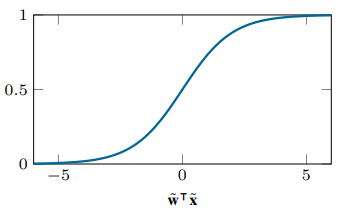
\includegraphics[width = 0.5\textwidth]{figs/sigmoidal.png}
\end{figure}  

Ejercicio: dado un modelo de clasificación binario lineal bidimensional con los parámetros $\theta = (b, \vec{w})$ con $b=1$ y $\vec{w} = (1,2)^T$ y los siguientes datos, computa la precisión:
\begin{itemize}
\item Probabilidad de $\vec{x}_1$ pertenecer a la clase $\mathcal{C}_1$ para $\vec{x}_1 = (1,1)^T$.

$$1 + 1 \cdot 1 + 2 \cdot 1 = 4$$
$$1 / (1 + e^{-4}) = 0.98$$

\item Probabilidad de $\vec{x}_2$ pertenecer a la clase $\mathcal{C}_1$ para $\vec{x}_2 = (1,-2)^T$.

$$1 + 1 \cdot 1 + 2 \cdot -2 = -2$$
$$1 / (1 + e^{2}) = 0.119$$

\item Probabilidad de $\vec{x}_3$ pertenecer a la clase $\mathcal{C}_0$ para $\vec{x}_3 = (0,0)^T$.

$$1 + 1 \cdot 0 + 2 \cdot 0 = 1$$
$$1 - (1 / (1 + e^{-1}) )= 0.2689$$
\end{itemize}

\subsubsection{Optimización: Máxima verosimilitud y entropía cruzada}

La verosimilitud de los datos es una elección común para cuantificar la calidad de un modelo probabilístico:
$$
\mathcal{L}(\mathcal{D};\tilde{\mathbf{w}}) = \prod_{i=1}^{N} p(t_i|\tilde{\mathbf{x}}_i; \tilde{\mathbf{w}}) = \prod_{i=1}^{N} \underbrace{p(C_0|\tilde{\mathbf{x}}_i; \tilde{\mathbf{w}})^{1-t_i} p(C_1|\tilde{\mathbf{x}}_i; \tilde{\mathbf{w}})^{t_i}}_{\begin{cases} 
    p(C_0|\tilde{\mathbf{x}}_i; \tilde{\mathbf{w}}) & \text{si } t_i = 0, \\ 
    p(C_1|\tilde{\mathbf{x}}_i; \tilde{\mathbf{w}}) & \text{si } t_i = 1. 
\end{cases}}
$$

El error de Entropía Cruzada (CE) se define como el logaritmo negativo de la verosimilitud:
$$
CE(\tilde{\mathbf{w}}) = -\log\mathcal{L}(\mathcal{D};\tilde{\mathbf{w}})
$$
$$
= \sum_{i=1}^{N} \left( -(1 - t_i) \log(p(C_0|\tilde{\mathbf{x}}_i; \tilde{\mathbf{w}})) - t_i \log(p(C_1|\tilde{\mathbf{x}}_i; \tilde{\mathbf{w}})) \right)
$$
$$
= \sum_{i=1}^{N} \left( -(1 - t_i) \log(1 - \sigma(\tilde{\mathbf{w}}^{T}\tilde{\mathbf{x}}_i)) - t_i \log(\sigma(\tilde{\mathbf{w}}^{T}\tilde{\mathbf{x}}_i)) \right).
$$

Ejercicio: dado un modelo de clasificación binario lineal bidimensional con los parámetros $\theta = (b, \vec{w})$ con $b=1$ y $\vec{w} = (1,2)^T$ y los siguientes datos, computa la precisión:
$$(1,1; 1) \rightarrow 1 + 1 \cdot 1 + 1 \cdot 2 = 4 $$
$$p1 = 1 / (1 + e^{-4}) = 0.98$$
$$p0 = 1 - 0.98 = 0.02$$
$$\mathcal{L} = (0.98)^1 \cdot (0.02)^0 = 0.98$$

$$(1,-2; 0) \rightarrow 1 + 1 \cdot 1 + 2 \cdot -2 = -2 $$
$$p1 = 1 / (1 + e^{2}) = 0.119$$
$$p0 = 1 - 0.119 = 0.881$$
$$\mathcal{L} = (0.881)^1 \cdot (0.119)^0 = 0.881$$

$$(0,0; 0) \rightarrow 1 + 1 \cdot 0 + 2 \cdot 0 = 1 $$
$$p1 = 1 / (1 + e^{-1}) = 0.7311$$
$$p0 = 1 - 0.2689 = 0.2689$$
$$\mathcal{L} = (0.2689)^1 \cdot (0.7311)^0 = 0.2689$$

$$ML = 0.98 \cdot 0.881 \cdot 0.2689 = 0.23$$

El CE minimizado es el máximo de ML. El algoritmo de aprendizaje para entrenar un modelo de Regresión Logística Lineal consiste en resolver el problema:
$$\min_{\tilde{\mathbf{w}} \in \mathbb{R}^{d+1}} \left\{ \mathrm{CE}(\tilde{\mathbf{w}}) \right\} = \min_{\tilde{\mathbf{w}} \in \mathbb{R}^{d+1}} \left\{ \sum_{i=1}^N \left( -(1-t_i) \log (1-\sigma(\tilde{\mathbf{w}}^{\intercal} \tilde{\mathbf{x}}_i)) - t_i \log (\sigma(\tilde{\mathbf{w}}^{\intercal} \tilde{\mathbf{x}}_i)) \right) \right\}.$$

Es convexa: no existen mínimos locales. Es diferenciable: los óptimos se caracterizan por los ceros del gradiente.

$$\nabla_{\tilde{\mathbf{w}}} \text{CE}(\tilde{\mathbf{w}})=\sum^N_{i=1} (\sigma (\tilde{\mathbf{w}}^T \tilde{\mathbf{x}}_i) - t_i) \tilde{\mathbf{x}}_i = \mathbf{0}
$$

El problema es que no siempre se puede igualar el gradiente a 0.

El Descenso Gradiente es un algoritmo de optimización simple (pero útil) que se utiliza a menudo en Aprendizaje Automático para encontrar el mínimo local.

\begin{figure}[h]
\centering
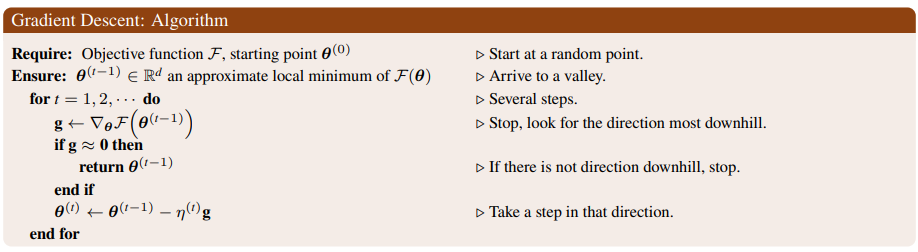
\includegraphics[width = \textwidth]{figs/gradient-descend-alg.png}
\end{figure}

El tamaño del paso $\eta^{(t)}$ debe fijarse en cada iteración t. Se trata de una cuestión crucial: Si el tamaño del paso es demasiado pequeño, el algoritmo necesitará demasiadas épocas (iteraciones) para converger y puede quedar atrapado en mínimos locales más fácilmente. Si el tamaño del paso es grande, la convergencia también será lenta. Si el tamaño del paso es demasiado grande, el descenso de gradiente sobrepasará los mínimos y divergirá. En algunos casos, se pueden calcular tamaños de paso óptimos.
Existen heurísticos que garantizan la convergencia, pero sólo a mínimos locales, y normalmente de forma lenta y zigzagueante.